\newpage
\section[Light as Electromagnetic Waves]{Light as Electromagnetic Waves (光是电磁波)}

\subsection{Unifying Light and Electromagnetic Waves}

\subsubsection{Review}

\begin{enumerate}
    \item Guass's law
    \begin{align*}
        \nabla \vec{E }=&\frac{\rho}{\epsilon_0}\\
        \nabla \vec{B}=&0
    \end{align*}
    \item Faraday
    \begin{align*}
        \nabla \times \vec{E}+\frac{\partial \vec{B }}{\partial t}=0
    \end{align*}
    \item Ampere-maxwell
    \begin{align*}
        \nabla \times \vec{B }-\mu_0 \epsilon_0\frac{\partial\vec{E }}{\partial t}=\vec{j}
    \end{align*}
\end{enumerate}

Without change or current (in vacuum (真空))

\begin{align*}
    \nabla^2 \vec{E}=&\frac{1}{c^2}\frac{\partial^2\vec{E}}{\partial t^2}\\
    \nabla^2\vec{B}=&\frac{1}{c }\frac{\partial^2\vec{B }}{\partial t^2}
\end{align*}

\subsubsection{Plane Wave}

Dimension (量纲)
\begin{itemize}
    \item $[c]=[\frac{[distance]}{[time]}]$
    \item $[\frac{\partial ^2}{\partial t^2}]=\frac{1}{[time]^2}$
    \item $[\nabla^2]=[\frac{\partial ^2}{\partial x^2}+\frac{\partial ^2}{\partial y^2}+\frac{\partial ^2}{\partial z^2}]=\frac{1}{[length^2]}$
\end{itemize}

Dimension (维度)
\begin{enumerate}
    \item one space dimension (scalar field (标量场)) \begin{align*}
        c^2\frac{\partial ^2}{\partial x^2}f(x, t)=\frac{\partial ^2}{\partial t^2}f(x, t)\\
        f(x, t)=f(x-ct)\\
        f(x,t)=f_0 \cos \left( kx-\omega t + \phi \right)
        , \,k=\frac{2\pi }{\lambda}, \, \omega=\frac{2 \pi }{T}
    \end{align*}
    \item three space dimension (vector field (矢量场))\begin{align*}
        \vec{E }(x,t) =\vec{E }_m \cos (\vec{k }\cdot\vec{r }-\omega t+\phi)\\
        \vec{B }(x,t) =\vec{B }_m \cos (\vec{k }\cdot\vec{r }-\omega t+\phi)
    \end{align*}
\end{enumerate}

\begin{figure}[H]
    \centering
    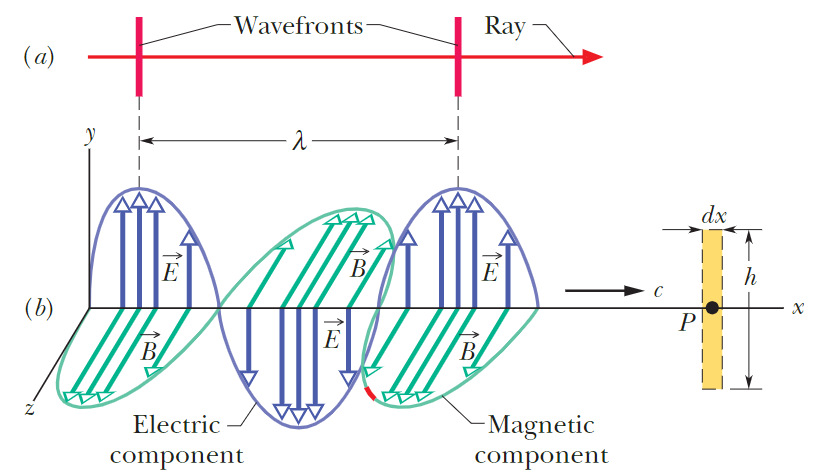
\includegraphics[width=0.309\textwidth]{Lec15/Plane Wave}
    \caption{Plane Wave}
\end{figure}

\subsubsection{Wavefronts}
At any instant a wavefront is a surface of constant phase. For the plane wave such a surface is
\begin{align*}
    \vec{k }\cdot \vec{r }=constant
\end{align*}

\subsection[The Propagation of Light Rays]{The Propagation of Light Rays (光传播)}
Called geometrical optics (几何光学). 
\subsubsection{Transmission of Light in Matter}
\begin{enumerate}
    \item the relative permittivity (相对介电常数) also called the dielectric constant $k/\epsilon_r$
    \item the relative permeability (相对渗透性) $\mu_r$
\end{enumerate}

A light wave propagating through any substantive medium travels at a speed
\begin{align*}
    v=\frac{1}{\sqrt{\epsilon_r \mu_r}}\frac{1}{\sqrt{\epsilon_0 \mu_0}}=\frac{c }{n }
\end{align*}
where the index of refracton $n=\sqrt{\epsilon_r \mu_r}$. 

The dispersion relation (散射率) becomes
\begin{align*}
    \omega=vk=\frac{ck }{n}    
\end{align*}
hence $k=nk_0$, where $k_0$ is the wave number in vacuum.

\subsubsection{Reflection and Refraction}
\begin{figure}[H]
    \centering
    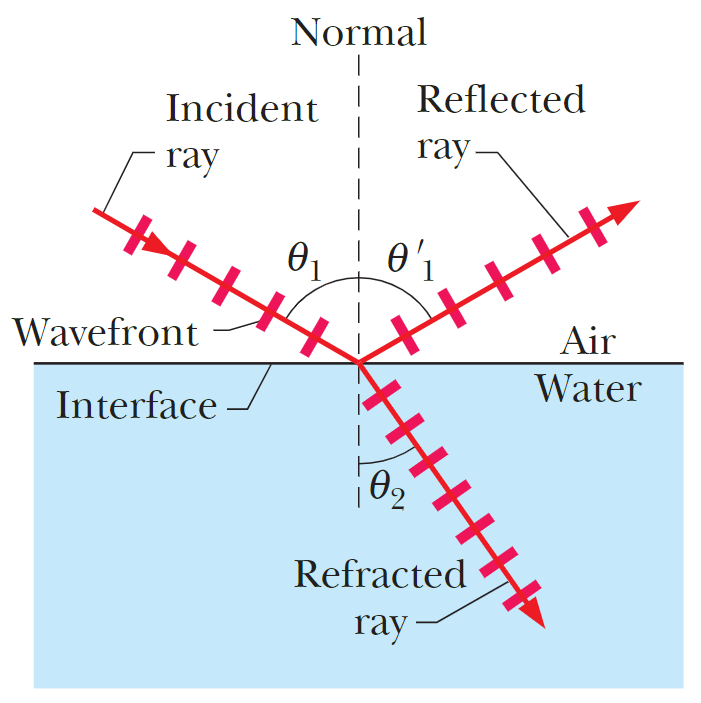
\includegraphics[width=0.2\textwidth]{Lec15/Reflection and Refraction}
    \caption{Reflection and Refraction}
\end{figure}

\begin{enumerate}
    \item Law of reflection: $\theta_1^{\prime}=\theta_1$. 
    \item Law of refraction (or Snell's law): $n_2\sin\theta_2=n_1\sin\theta_1$. 
\end{enumerate}

\subsubsection{Total Internal Reflection}
\begin{figure}[H]
    \centering
    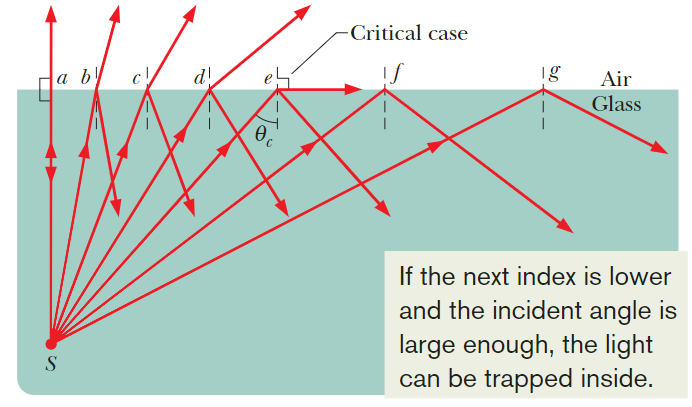
\includegraphics[width=0.31\textwidth]{Lec15/Total Internal Reflection}
    \caption{Total Internal Reflection}
\end{figure}

At a critical (临界) $\theta_0$ , the refracted ray points directly along the interface, i.e.
\begin{align*}
    n_{glass}\sin\theta_c=n_{air}\sin\left( \frac{\pi}{2} \right)
\end{align*}
For larger $\theta$, all the light is reflected. 

\subsection{Understanding the Laws of Reflection and Refraction}

\subsubsection{Fermat's Principle}
The principle of least time: The actual path between two points taken by a beam of light is the one that is traversed in the least time (光路径最短, 走直线). 

\begin{figure}[H]
    \centering
    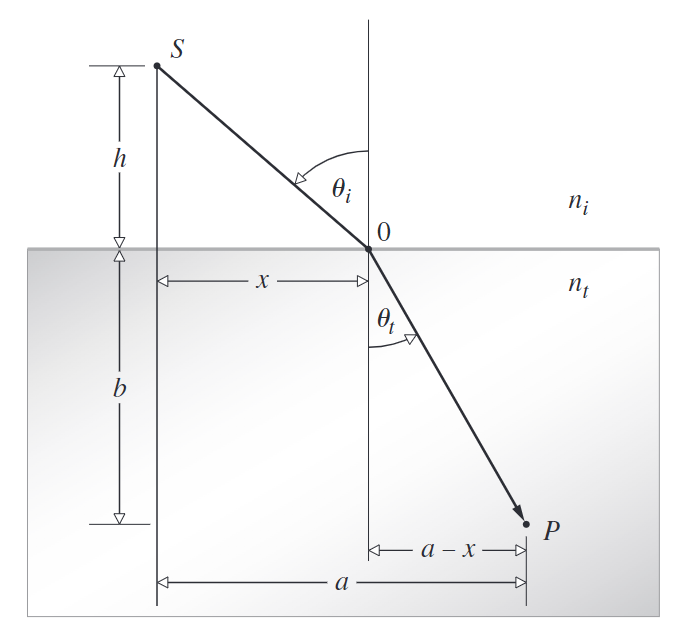
\includegraphics[width=0.2\textwidth]{Lec15/Fermat's Principle}
    \caption{Fermat's Principle}
\end{figure}

\begin{align*}
    &t=\frac{\overrightarrow{SO }}{v_i }+\frac{\overrightarrow{OP }}{v_t }, \text{ Let } \frac{dt }{dx }=0\\
    \therefore& n_i\sin \theta_i = n_t \sin \theta_t
\end{align*}

The Mirage (海市蜃楼) with Fermat’s Principle: 
\begin{figure}[H]
    \centering
    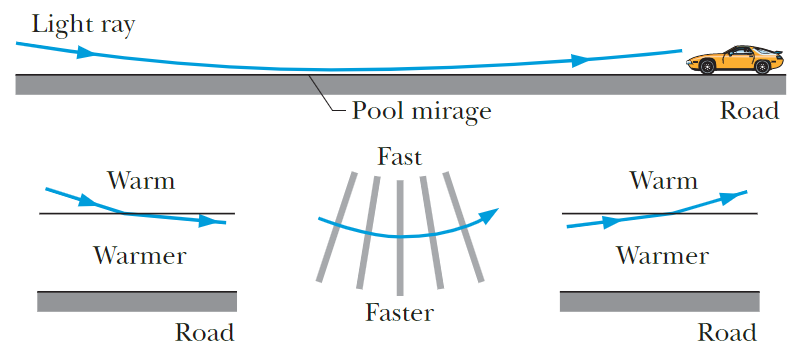
\includegraphics[width=0.31\textwidth]{Lec15/Mirage}
    \caption{Mirage}
\end{figure}

\subsubsection{Huygens' Principle}
All points on a wavefront serve as point sources of spherical secondary wavelets. After a time t, the new position of the wavefront will be that of a surface tangent to these secondary wavelets. 

\begin{figure}[H]
    \centering
    \begin{subfigure}{0.155\textwidth}
        \centering
        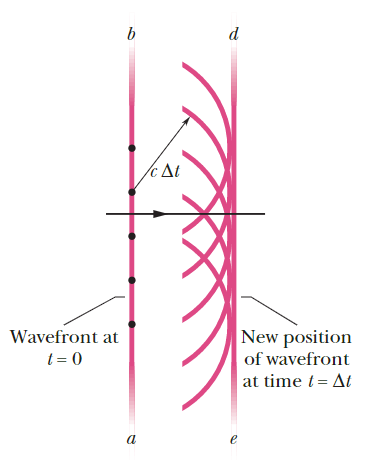
\includegraphics[width=\textwidth]{Lec15/Huygens' Principle}
        % \caption{Huygens' Principle}
    \end{subfigure}
    \begin{subfigure}{0.31\textwidth}
        \centering
        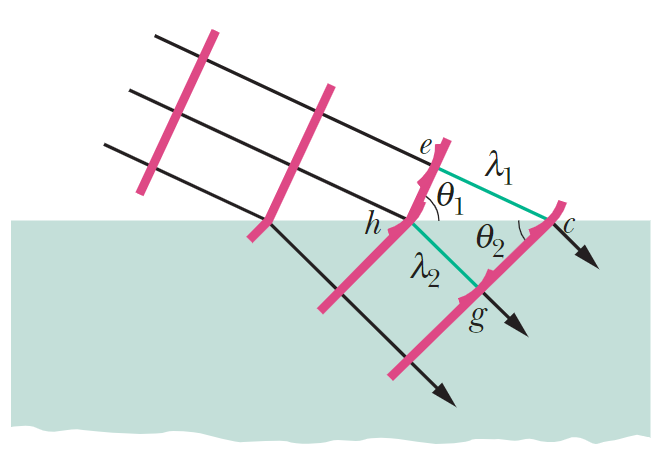
\includegraphics[width=\textwidth]{Lec15/Huygens' Principle 2}
        % \caption{Huygens' Principle 2}
    \end{subfigure}
    \caption{Huygens' Principle}
\end{figure}
 
\begin{align*}
    \because \, &\frac{\lambda_1}{\lambda_2}=\frac{v_1}{v_2}\\
    & \sin \theta_1=\frac{\lambda_1}{hc}, \, \sin\theta_2=\frac{\lambda_2}{hc}\\
    \therefore \, & \frac{\sin \theta_1}{\sin \theta_2}=\frac{\lambda_1}{\lambda_2}=\frac{v_1}{v_2}=\frac{\frac{c }{n_1 }}{\frac{c }{n_2 }}=\frac{n_2 }{n_1}\\
    \text{or }& n_2\sin\theta_2=n_1\sin\theta_1
\end{align*}

\subsubsection{The Electromagnetic Approach}
Suppose that the incident, reflected, and transmitted ($\vec{E}_i, \vec{E}_r, \vec{E}_t$, 入射波, 反射波, 透射波) waves can be written as
\begin{align*}
    \vec{E}_i=&\vec{E}_{0i}\cos\left( \vec{k}_i\cdot\vec{r}-\omega_i t \right)\\
    \vec{E}_r=&\vec{E}_{0r}\cos\left( \vec{k}_r\cdot\vec{r}-\omega_r t +\phi_r\right)\\
    \vec{E}_t=&\vec{E}_{0t}\cos\left( \vec{k}_t\cdot\vec{r}-\omega_t t +\phi_t\right)
\end{align*}
$\vec{k}$ is space angular velocity. 

So we have $\vec{E}=\vec{E}_i+\vec{E}_r$ above the interface and $\vec{E}=\vec{E}_t$ below. For simplicity, we consider the case that $\vec{E}_{0i}, \vec{E}_{0r}, \vec{E}_{0t}$ are constant in time. 

\begin{figure}[H]
    \centering
    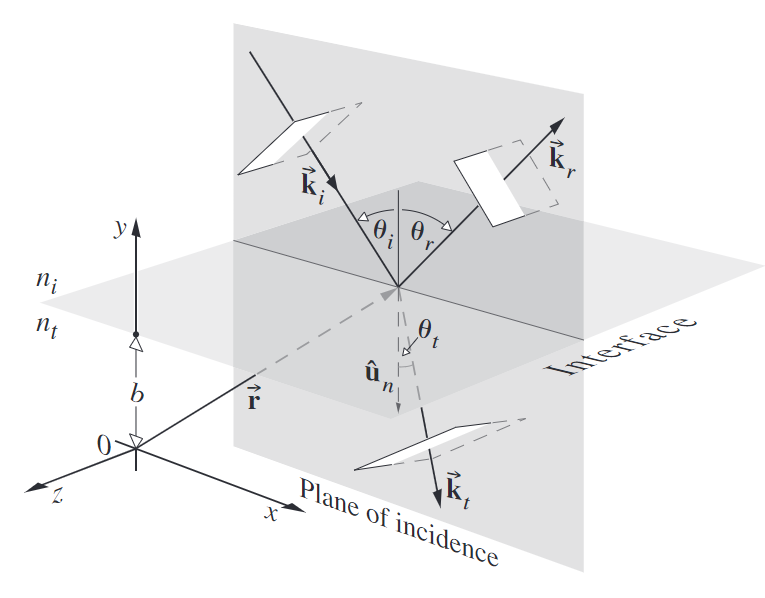
\includegraphics[width=0.309\textwidth]{Lec15/The Electromagnetic Approach}
    \caption{The Electromagnetic Approach}
\end{figure}

The laws of electromagnetic theory lead to certain requirements that must be met by the fields, and they are referred to as the \highlight{boundary conditions} (边界条件). 

\begin{figure}[H]
    \centering
    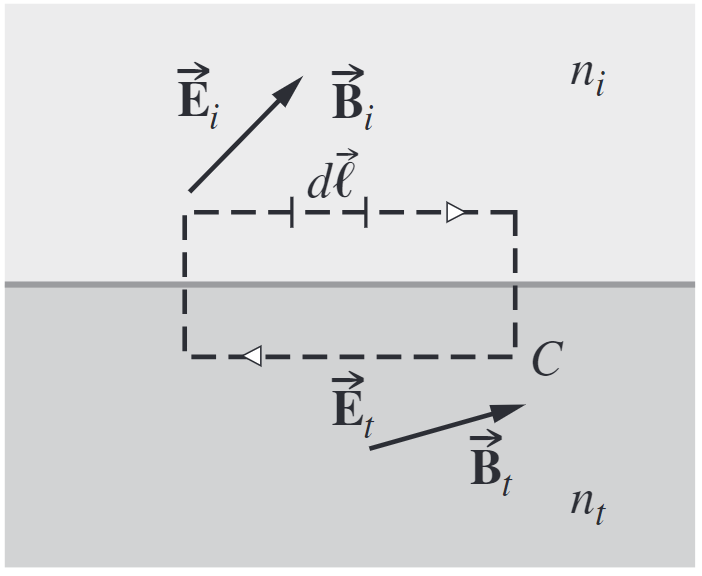
\includegraphics[width=0.21\textwidth]{Lec15/the boundary conditions}
    \caption{the boundary conditions}
\end{figure}

For example, we draw a narrow closed path $C$ that runs parallel to the interface inside both media. According to Faraday's induction law 
\begin{align*}
    \oint \vec{E}\cdot \mathrm{d} \vec{s}=-\frac{\mathrm{d }\Phi_B }{\mathrm{d}t}
\end{align*}

The loop can be made so narrow such that there is no flux
through $C$ . Define $\hat{u}_n$ to be the unit vector normal to the interface. The boundary condition leads to
\begin{align*}
    \hat{u}_n \times (\vec{E}_i+\vec{E}_r)-\hat{u}_n \times \vec{E}_t=0
\end{align*}
which is satisfied for all values of time and at any point on the interface. That is 
\begin{align*}
    &\hat{u}_n \times \vec{E}_{0i}\cos\left( \vec{k}_i\cdot\vec{r}-\omega_i t \right)\\
    +& \hat{u}_n \times \vec{E}_{0r}\cos\left( \vec{k}_r\cdot\vec{r}-\omega_r t +\phi_r\right) \\
    =& \hat{u}_n \times \vec{E}_{0t}\cos\left( \vec{k}_t\cdot\vec{r}-\omega_t t +\phi_t\right)
\end{align*}

This can only be satisfied if $\omega_i=\omega_r=\omega_t$, which means \highlight{the charged particles (带电粒子) within the media are undergoing force oscillations (振荡) at the frequency of the incident wave }. 

Furthermore, for any $\vec{r}$ terminating on the interface
\begin{align*}
    \left. \left( \vec{k}_i \cdot \vec{r} \right)\right|_{y=b} = \left. \left( \vec{k}_r \cdot \vec{r} +\phi_r \right)\right|_{y=b} = \left. \left( \vec{k}_i \cdot \vec{r} +\phi_t \right)\right|_{y=b}
\end{align*}

Thus, we find
\begin{align*}
    &\left[ (\vec{k}_i-\vec{k}_r)\cdot \vec{r} \right]=\phi_r\\
    \text{or }&(\vec{k}_i-\vec{k}_r)\cdot(\vec{r}_1-\vec{r}_2)=0
\end{align*}
for any pair of $\vec{r}_1$ and $\vec{r}_2$ terminating on the interface. 

And we also have $\hat{u}_n\cdot(\vec{r}_1-\vec{r}_2)=0$, so $(\vec{k}_i-\vec{k}_r)$ is parallel to $\hat{u}_n$, or $k_i\sin\theta_i=k_r\sin\theta_r$. 

Since the incident and reflected waves are in the same medium, $k_i=k_r$, so finally, $\theta_i=\theta_r$. 

Similarly, $(\vec{k}_i-\vec{k}_t)$ is also parallel to $\hat{u}_n$, 
\begin{align*}
    \vec{k}_i\times \hat{u}_n=\vec{k}_t\times \hat{u}_n
\end{align*}
or (notice $\vec{k}=nk_0\hat{k}$)
\begin{align*}
    n_i\left( \hat{k}_i\times \hat{u}_n \right)=n_t\left( \hat{k}_t\times \hat{u}_n \right)
\end{align*}
which is nothing but the law of refraction. 

Note that the law of reflection and the law of refraction only rely on the \highlight{phase relationship (相位关系) that exists among the phases of $\vec{E}_i$, $\vec{E}_r$ and $\vec{E}_t$ at the boundary}. 

There is still an interdependence shared by the amplitudes $\vec{E}_{0i}$, $\vec{E}_{0r}$ and $\vec{E}_{0t}$. The additional constraint can be used to calculate the amplitude of the reflected wave and the transmitte wave (the Fresnel equations). This will lead to the phenomenon of polarization by reflection. 

\subsubsection{Light in Another Inertial Frame}
A light wave looks like a light wave in any inertial frame of reference.

用Maxwell导出光速不变, 光速不变又是相对论基础. 